\documentclass[../DoAn.tex]{subfiles}
\begin{document}

% 2.1 Khảo sát hiện trạng
\section{Khảo sát hiện trạng}
\label{section:2.1}
Để hoàn thành mục tiêu đề tài đã nêu ra ở chương \ref{chapter:Introduction}, đó là xây dựng một hệ thống quản lý dự án, trước hết, việc khảo sát các phần mềm tương tự và
phổ biến hiện nay là một điều cần thiết, nhằm tìm ra những tính năng cốt lõi và thiết yếu của hệ thống. Trong phần này, em sẽ tìm hiểu về hai phần mềm là Asana và Azure Devops.

%% 2.1.1 Asana
\label{subsection:2.1.1}
\subsection{Asana}
Asana là một trong những phần mềm quản lý dự án phổ biến nhất trên thị trường hiện này, với nhiều tính năng nổi bật, tập trung vào việc tuỳ chỉnh linh hoạt các dự án, và tương tác giữa các thành viên trong cùng một đội. Về các tính năng cơ bản, công cụ này cho phép các đội nhóm tạo ra các dự án,
quản lý công việc chung, theo dõi tiến độ của dự án, và giao tiếp với nhau thông qua các bình luận, thảo luận. Ngoài ra, người dùng có thể đăng ký một tổ chức bao gồm nhiều
đội nhóm, dự án khác nhau, chúng có thể tương tác qua lại lẫn nhau, giúp chia nhỏ công việc cho các đội nhóm từ 4-8 thành viên, dễ dàng hơn trong việc quản lý.

Về điểm mạnh, Asana được thiết kế dựa trên Agile, một phương pháp luận phổ biến trong ngành phát triển phần mềm hiện nay. Chính vì vậy, công cụ này cung cấp cho người dùng
đa dạng sự lựa chọn về cách hiển thị dự án, từ dạng bảng Kanban, lịch, đến các biểu đồ thống kê, giúp họ có thể dễ dàng theo dõi tiến độ của dự án một cách nhanh chóng.
Các tổ chức, công ty phần mềm lớn dễ dàng có thể tích hợp Asana vào quy trình phát triển sản phẩm của mình.

Asana còn hỗ trợ tốt trong việc tích hợp với các phần mềm bên thứ ba phổ biến về tự động hoá và quản lý đội nhóm, ví dụ như Slack và Zapier. Các phần mềm này được sử dụng nhiều
trong quy trình làm việc của các công ty, nhờ đó, luồng thông tin giữa các thành viên được đồng bộ, giảm thiểu tối đa việc trùng lặp hay bỏ sót thông tin quan trọng khi phải
làm việc trên đa nền tảng.

Về điểm yếu, Asana không có một hệ sinh thái các phần mềm doanh nghiệp so với các đối thủ, như Azure Devops của Microsoft hay Jira của Atlassian.
Điều này khiến cho nhân viên của các công ty lớn phải quản lý nhiều hơn một tài khoản doanh nghiệp, một số thông tin nội bộ không thể chia sẻ với một nền tảng đám mây khác
do chính sách bảo mật. Ngoài ra, mức giá giá của Asana cũng là một rào cản lớn đối với các công ty nhỏ, đội nhóm làm việc tự do trong khi phiên bản miễn phí của Asana rất
hạn chế về tính năng.



%% 2.1.2 Azure Devops
\label{subsection:2.1.2}
\subsection{Azure Devops}
Azure Devops là một nền tảng quản lý dự án, phát triển phần mềm, được phát triển bởi Microsoft. Nền tảng này cho phép người dùng quản lý một quy trình phát triển phần mềm
khép kín, từ việc quản lý mã nguồn, kiểm thử, triển khai, đến việc theo dõi tiến độ của dự án.

Về điểm mạnh, Azure Devops hoàn toàn được thiết kế cho việc vận hành một dự án phát triển phần mềm theo phương pháp Agile, đặc biệt là mô hình Scrum, một bộ khung được dựa
trên phương pháp Agile, chỉ ra các vai trò, sự kiện và nguyên tắc trong một quy trình phát triển phần mềm. Các tính năng của công cụ này đều dựa trên các khái niệm của Agile và Scrum,
giúp cho các tổ chức, công ty phần mềm có thể vận hành một quy trình phát triển phần mềm hiệu quả, đơn giản hơn theo mô hình này.

Azure Devops còn cung cấp các công cụ khác trong việc phát triển một phần mềm, qua đó, các công việc được liên kết với các thay đổi trong mã nguồn, kết quả kiểm thử,
và các tài liệu kỹ thuật liên quan. Vì vậy, việc truy vết, tra cứu các thông tin liên quan đến một công việc, một tính năng trong sản phẩm phần mềm có thể được thực hiện
một cách nhanh chóng, đầy đủ thông tin ở trên duy nhất một nền tảng.

Ngoài ra, vì là một nền tảng được phát triển bởi Microsoft, các tổ chức, công ty phần mềm có thể dễ dàng quản lý các tài khoản, dữ liệu liên quan đến dự án cùng với
các ứng dụng phần mềm văn phòng, quản trị tổ chức khác của họ.

Về điểm yếu, Azure Devops là một phần mềm có quá nhiều tính năng nhưng lại kém linh hoạt, ít khả năng tuỳ chỉnh, khiến cho việc sử dụng có thể trở nên phức tạp.
Trong một số trường hợp, các tính năng này trở nên không cần thiết với tổ chức, công ty không sử dụng hệ sinh thái ứng dụng của Microsoft, hoặc họ có nhu cầu sử dụng
một quy trình phần mềm khác, không phải Agile, Scrum. Tuy nhiên, Microsoft lại hướng Azure Devops đến các tổ chức, công ty phần mềm lớn, có số lượng nhân viên lớn,
quy trình phát triển phần mềm cụ thể, có yêu cầu cao trong việc bảo mật, quản trị dữ liệu, tài khoản, và các ứng dụng phần mềm khác của họ.

Hơn hết, tuy nền tảng này cung cấp rất nhiều công cụ, hỗ trợ một quy trình phát triển phần mềm khép kín, song song với đó, không có công cụ nào trong số chúng là thực
sự đủ tốt so với các đối thủ khác. Ví dụ, với công việc quản lý mã nguồn, tự động kiểm thử và triển khai ứng dụng, GitHub và GitLab là hai nền tảng phổ biến và được
đánh giá tốt hơn nhiều so với Azure Devops.

% 2.2 Tổng quan chức năng
\section{Tổng quan chức năng}
\label{section:2.2}
Hệ thống được xây dựng phù hợp với các mô hình phát triển phần mềm hiện nay đặc biệt là mô hình Scrum.
Hệ thống phục vụ cho hai tác nhân chính là Người dùng (User) và Quản trị viên (Admin).

%% 2.2.1 Biểu đồ use case tổng quát
\subsection{Biểu đồ use case tổng quát}
\label{subsection:2.2.1}
Tác nhân người dùng có các chức năng như đăng nhập, đăng xuất, quản lý tổ chức, quản lý dự án, quản lý công việc. Tác nhân quản trị viên có các chức năng như đăng nhập,
đăng xuất và quản lý tài khoản. Tác nhân khách (Guest), là những tác nhân chưa phải người dùng của hệ thống, có chức năng là đăng ký tài khoản.
Các ca sử dụng sẽ được phân rã ở những mục tiếp theo.
\begin{figure}[H]
    \centering
    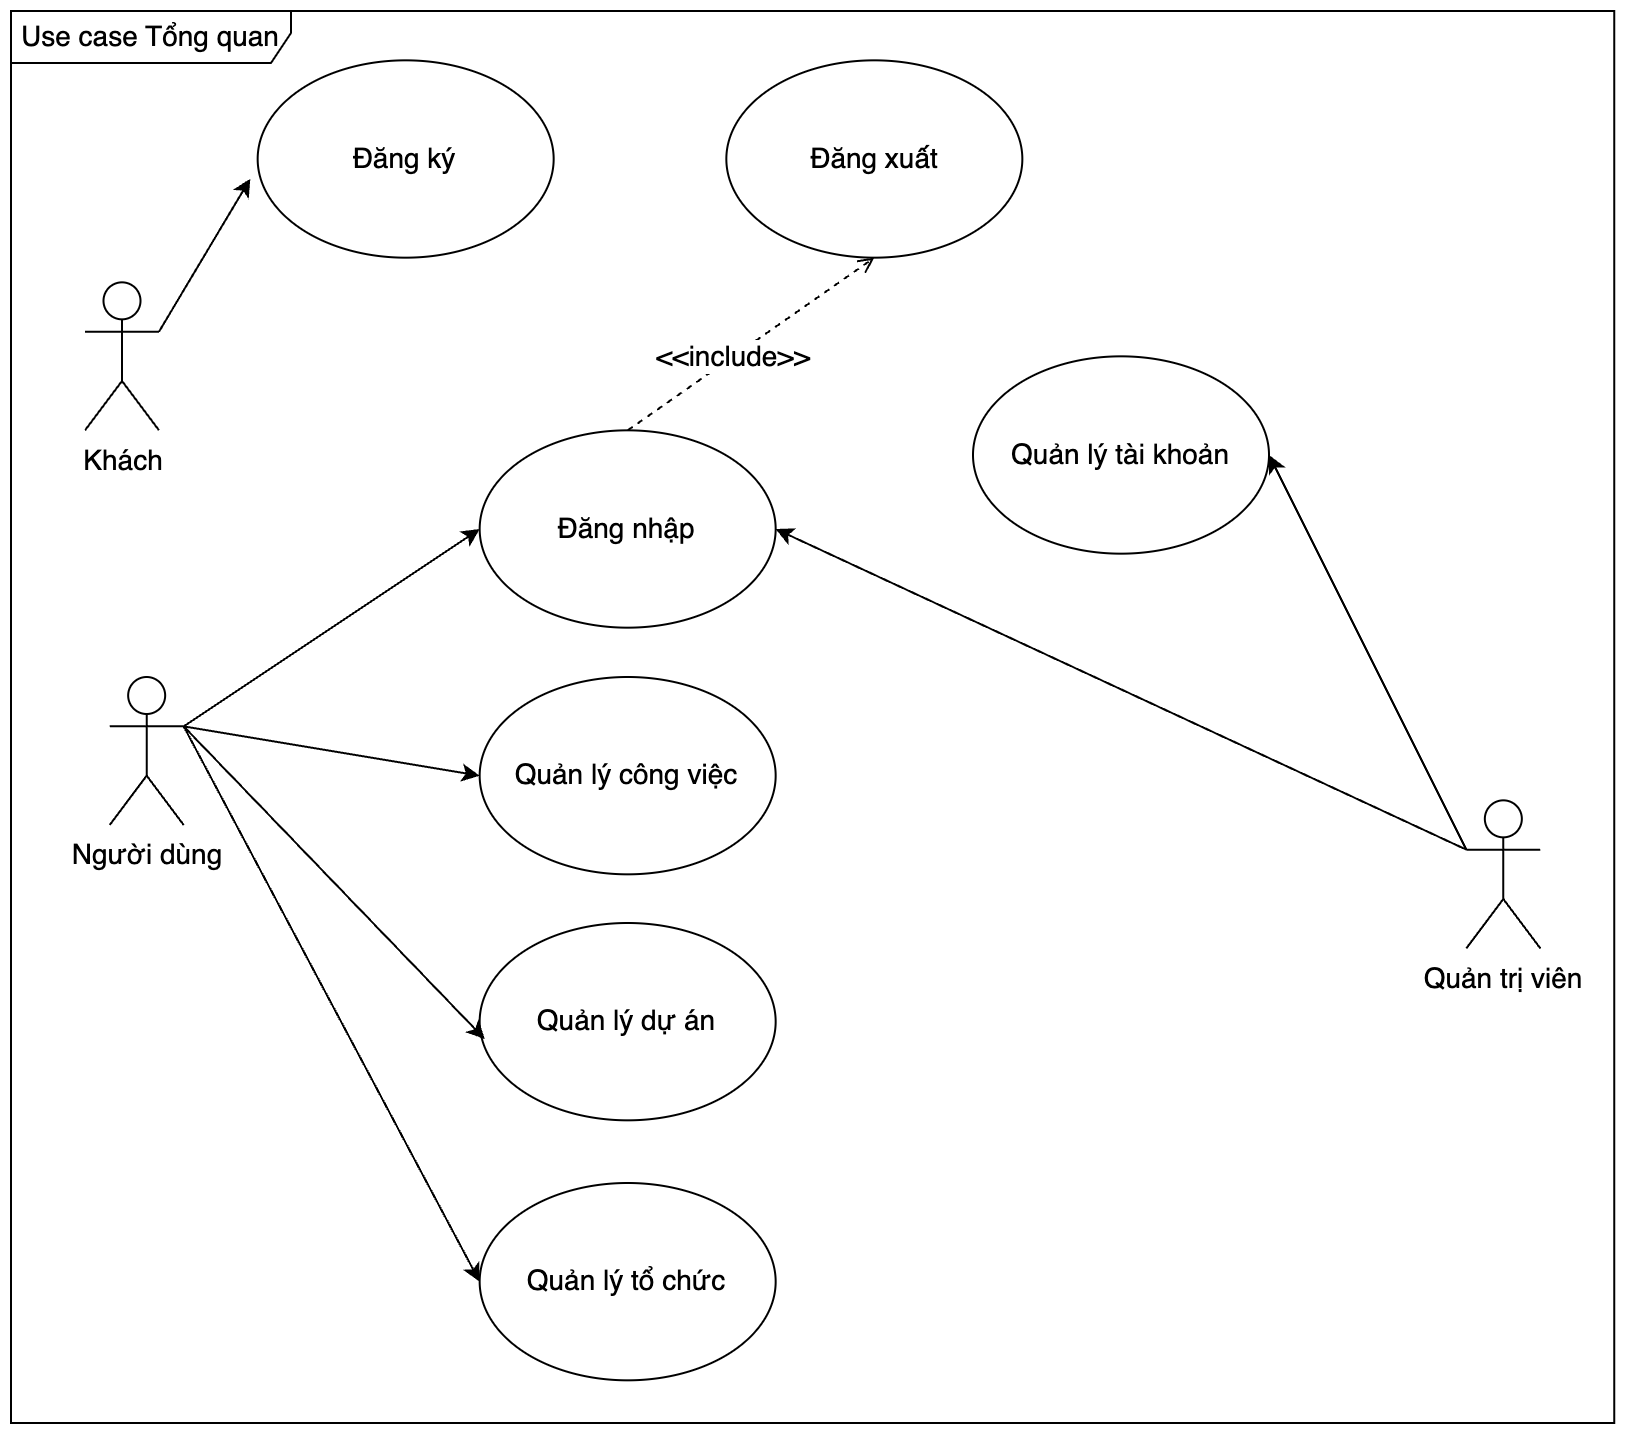
\includegraphics[width=1.0\linewidth]{Hinhve/GeneralUseCases.png}
    \caption{Biểu đồ use case tổng quát}
    \label{fig:GeneralUseCases}
\end{figure}
\newpage

%% 2.2.2 Biểu đồ use case phân rã Quản lý tài khoản
\subsection{Biểu đồ use case phân rã Quản lý tài khoản}
\label{subsection:2.2.2}
Use case Quản lý tài khoản với tác nhân chính là Quản trị viên bao gồm các chức năng chính là xem toàn bộ tài khoản, chỉnh sửa tài khoản, vô hiệu hoá tài khoản,
tái kích hoạt tài khoản và xem chi tiết tài khoản.
\begin{figure}[H]
    \centering
    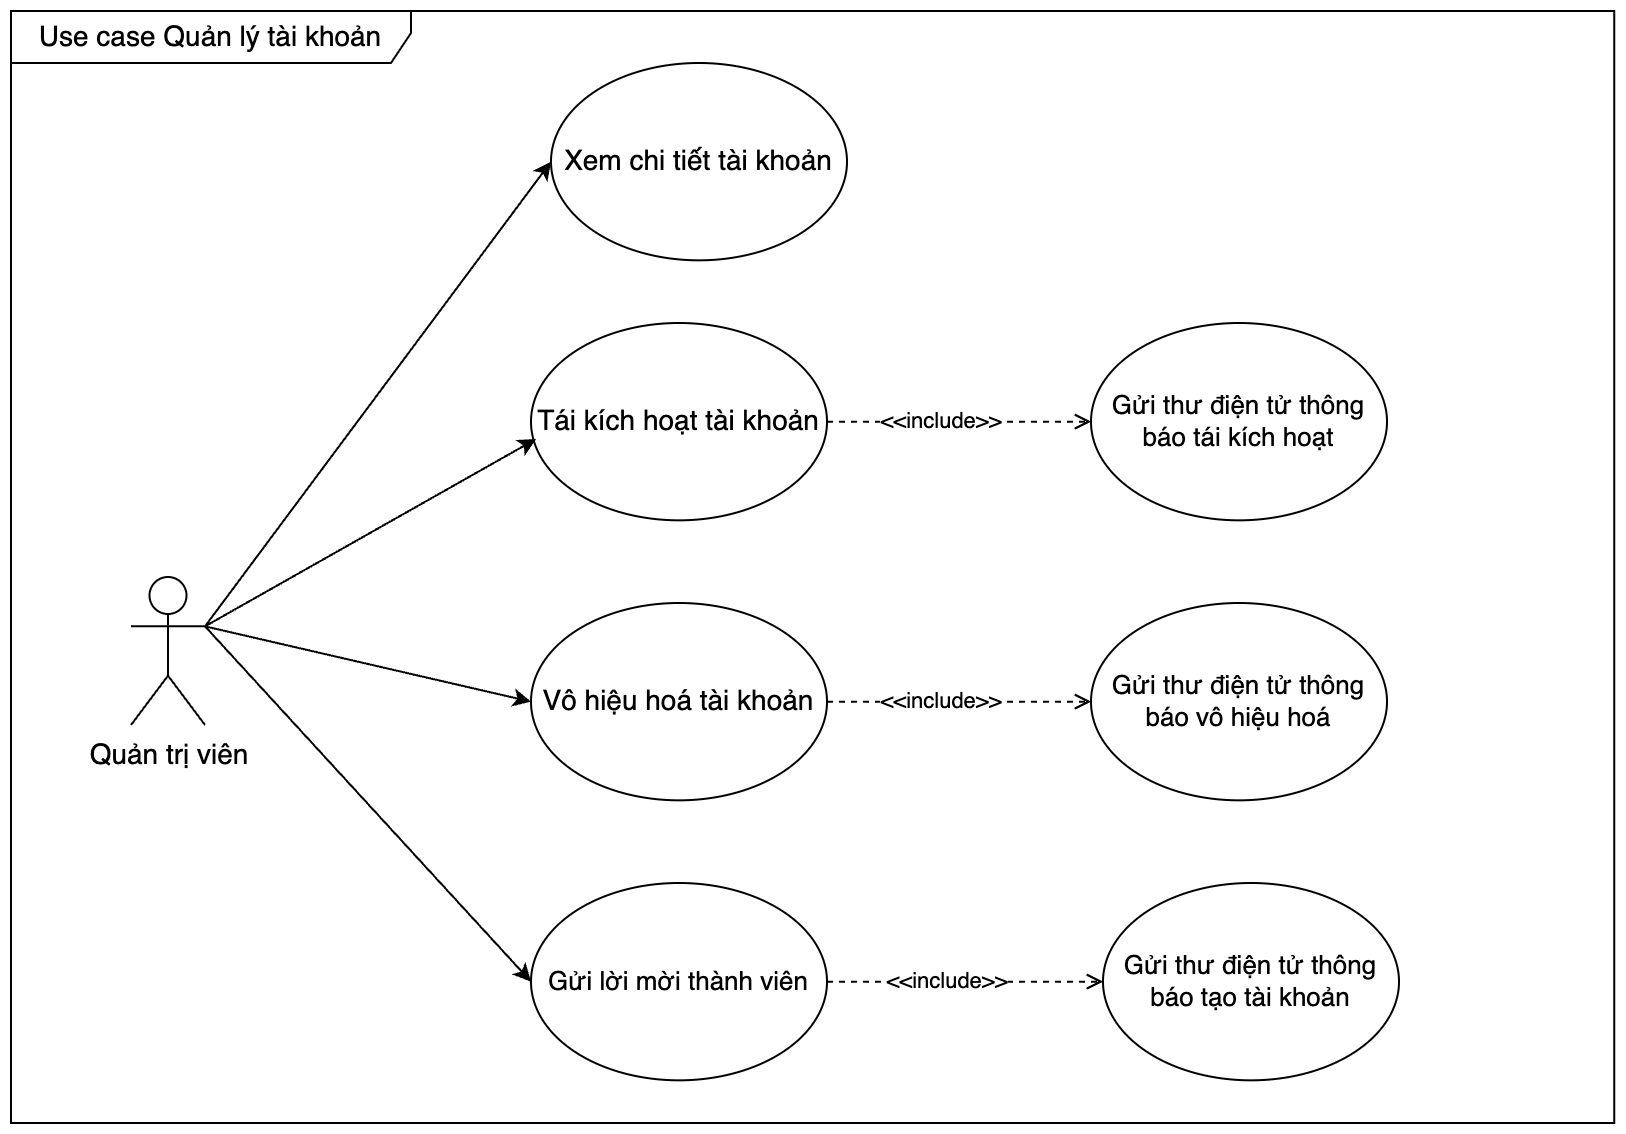
\includegraphics[width=1.0\linewidth]{Hinhve/AccountUseCases.png}
    \caption{Biểu đồ use case phân rã Quản lý tài khoản}
    \label{fig:AccountUseCases}
\end{figure}
\newpage

%% 2.2.3 Biểu đồ use case phân rã Quản lý tổ chức
\subsection{Biểu đồ use case phân rã Quản lý tổ chức}
\label{subsection:2.2.3}
Use case Quản lý lý tổ chức với tác nhân chính là Người dùng bao gồm các chức năng chính là quản lý thành viên, thêm tổ chức, chỉnh sửa thông tin tổ chức, xoá tổ chức
\begin{figure}[H]
    \centering
    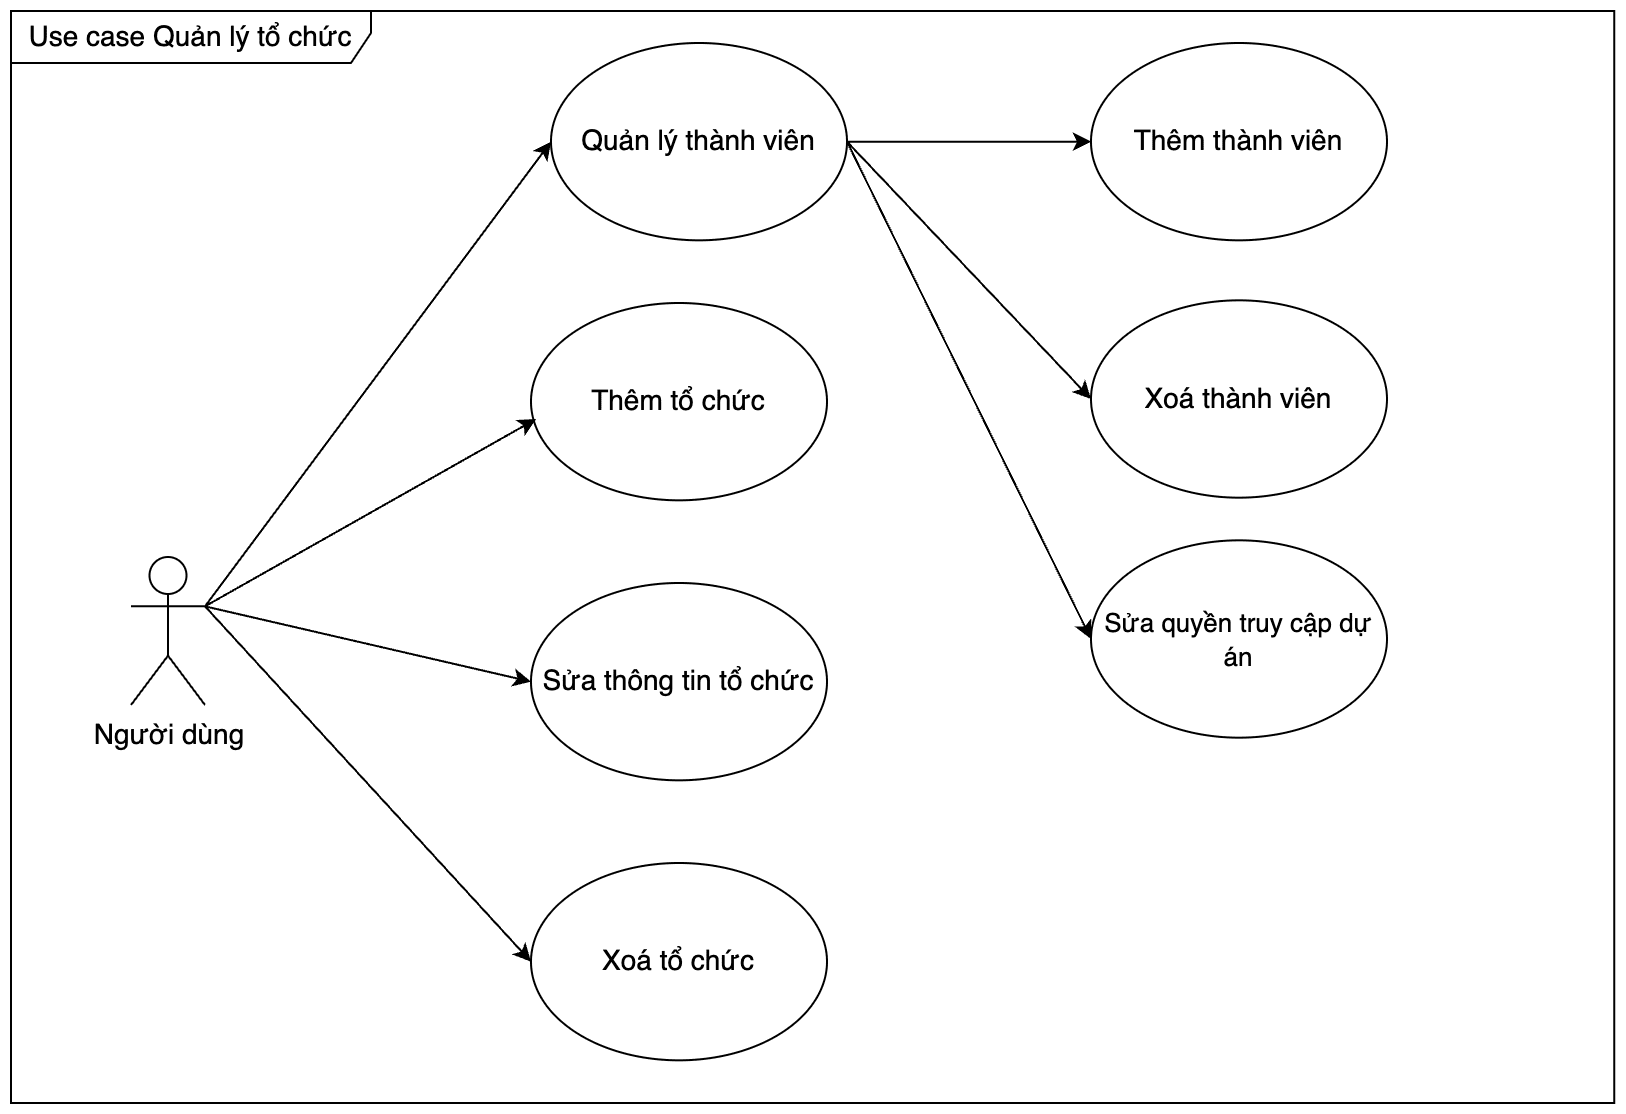
\includegraphics[width=1.0\linewidth]{Hinhve/WorkspaceUseCases.png}
    \caption{Biểu đồ use case phân rã Quản lý tổ chức}
    \label{fig:WorkspaceUseCases}
\end{figure}
\newpage

%% 2.2.4 Biểu đồ use case phân rã Quản lý dự án
\subsection{Biểu đồ use case phân rã Quản lý dự án}
\label{subsection:2.2.4}
Use case Quản lý dự án bao gồm các chức năng chính là thêm dự án, chinh sửa thông tin dự án, quản lý các thành viên trong dự án,
các milestones của dự án và các category của dự án.
\begin{figure}[H]
    \centering
    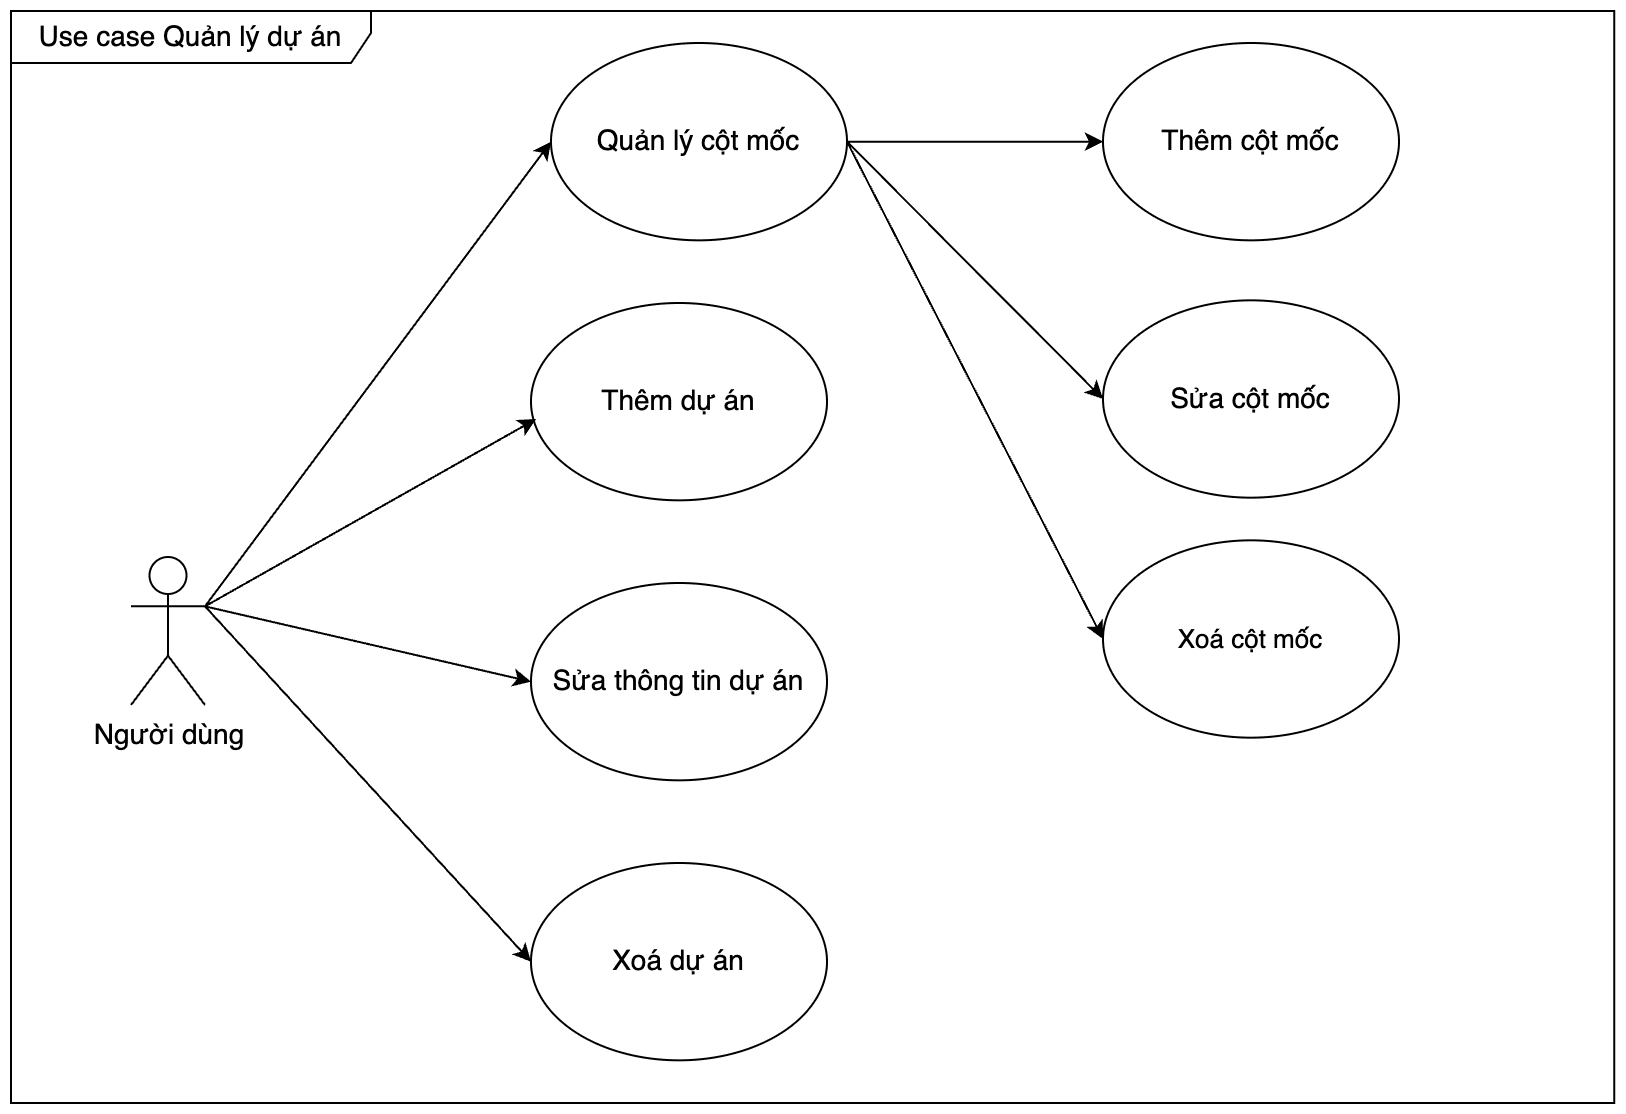
\includegraphics[width=1.0\linewidth]{Hinhve/ProjectUseCases.png}
    \caption{Biểu đồ use case phân rã Quản lý dự án}
    \label{fig:ProjectUseCases}
\end{figure}
\newpage

%% 2.2.5 Biểu đồ use case phân rã Quản lý công việc
\subsection{Biểu đồ use case phân rã Quản lý công việc}
\label{subsection:2.2.5}
Use case Quản lý công việc bao gồm các chức năng chính là thêm công việc, sửa thông tin công việc và xem danh sách công việc.
Trong sửa thông tin công việc chúng ta có thể thay đổi trạng thái của nó, giao công việc đó cho người khác.
Trong xem danh sách công việc có thể sử dụng chức năng lọc để xem danh sách công việc theo các thuộc tính như người được giao, milestone,
category và một vài thuộc tính khác.
\begin{figure}[H]
    \centering
    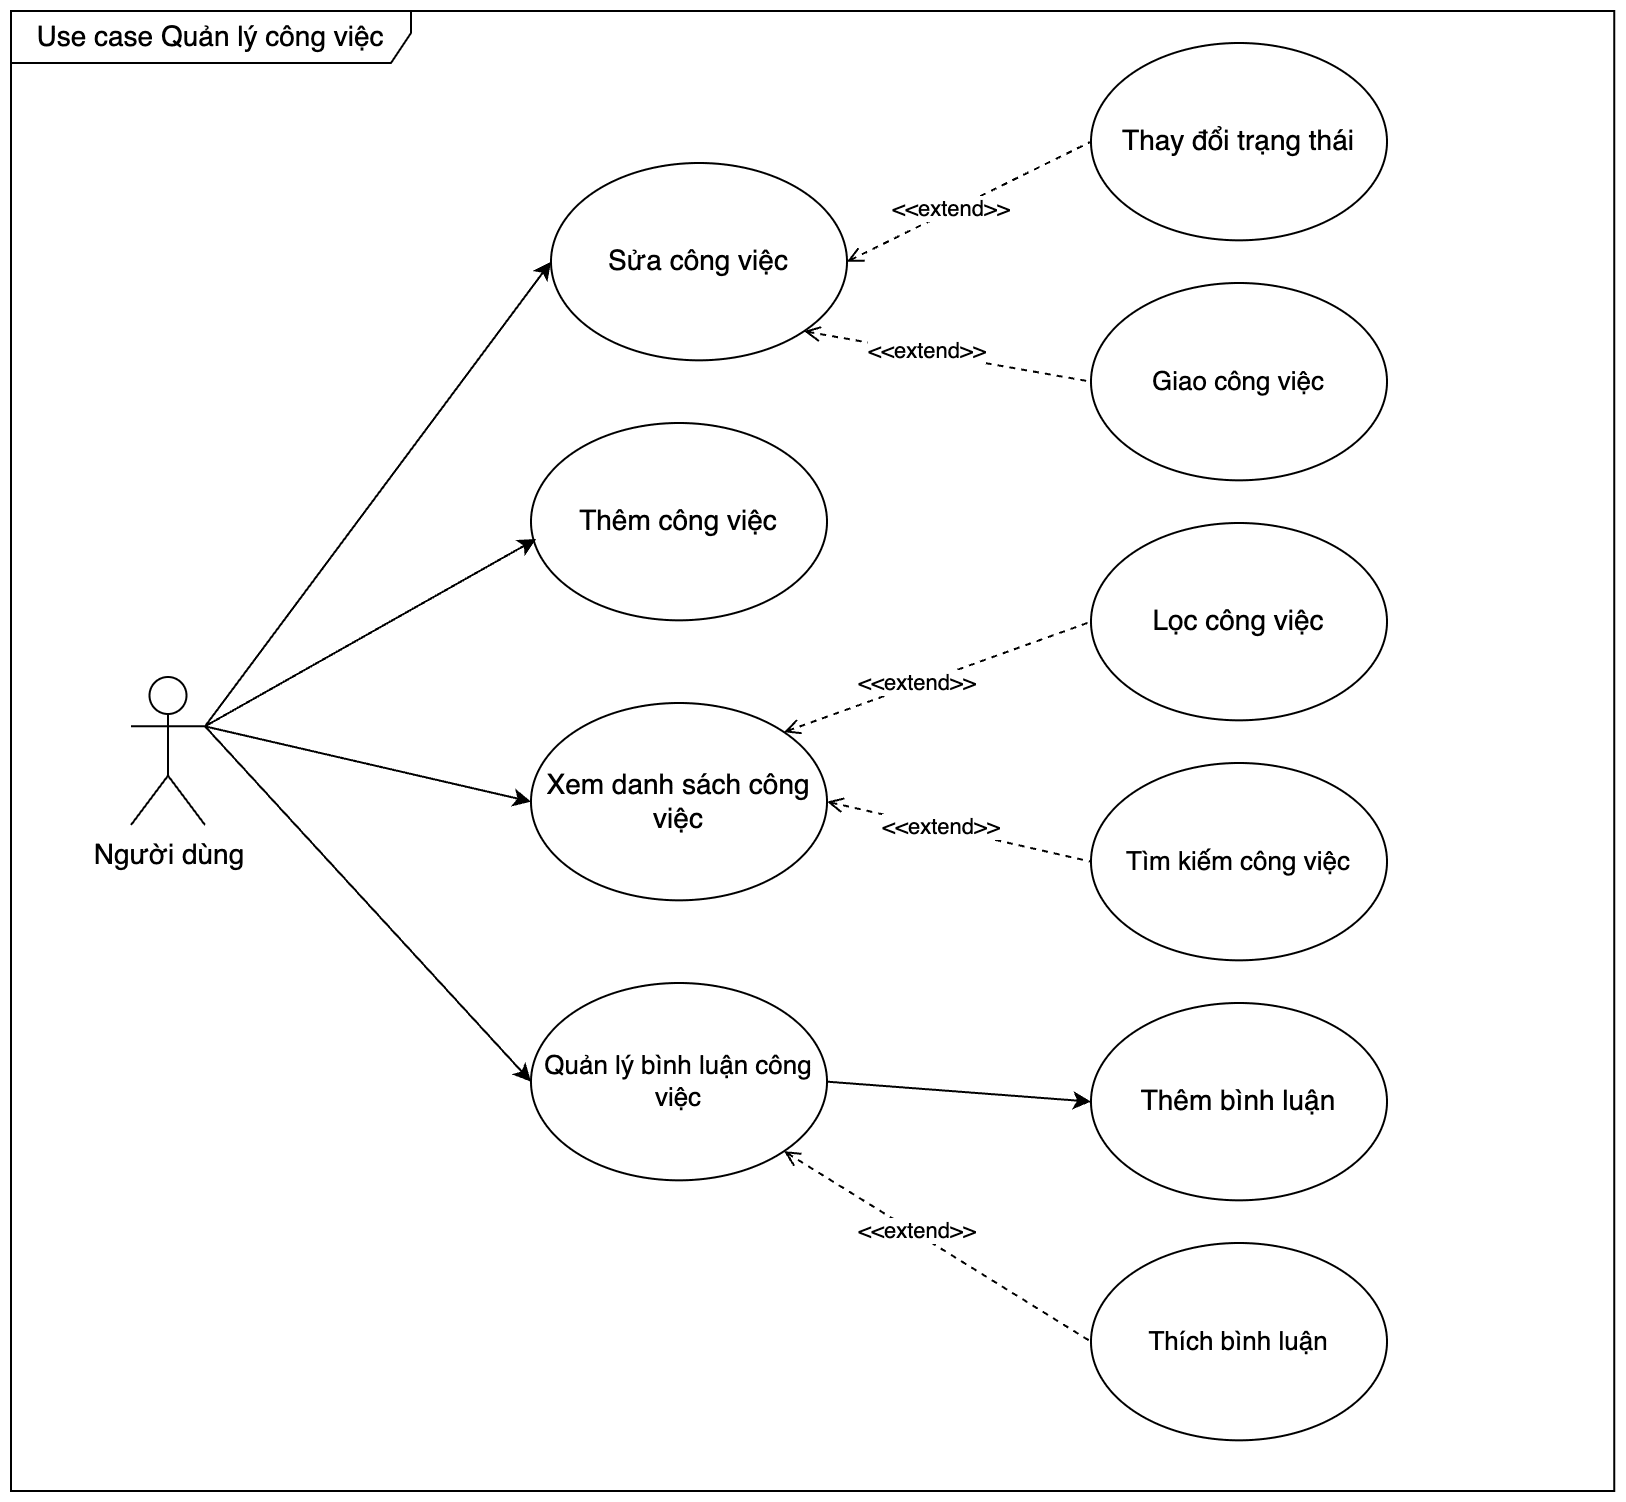
\includegraphics[width=1.0\linewidth]{Hinhve/TaskUseCases.png}
    \caption{Biểu đồ use case phân rã Quản lý công việc}
    \label{fig:TaskUseCases}
\end{figure}
\newpage

\section{Đặc tả chức năng}
\label{section:2.3}

\subsection{Đặc tả use case Đăng ký}
\label{subsection:2.3.1}

\begin{table}[ht]
    \renewcommand{\arraystretch}{1.2}
    \centering
    \begin{tabular}{| p{0.2\linewidth} | p{0.1\linewidth} | p{0.2\linewidth} | p{0.5\linewidth} |}
        \hline
        \textbf{Mã usecase}                                          & UC01                                                                                   & \textbf{Tên usecase}                                       & Đăng ký                                                                                                                 \\ \hline
        \multicolumn{1}{|p{0.2\linewidth}|}{\textbf{Tác nhân}}       & \multicolumn{3}{p{0.8\linewidth}|}{Khách}                                                                                                                                                                                                                                     \\ \hline
        \multicolumn{1}{|p{0.2\linewidth}|}{\textbf{Mô tả}}          & \multicolumn{3}{p{0.8\linewidth}|}{Ca sử dụng cho phép tác nhân tạo một tài khoản mới}                                                                                                                                                                                        \\ \hline
        \multicolumn{1}{|p{0.2\linewidth}|}{\textbf{Tiền điều kiện}} & \multicolumn{3}{p{0.8\linewidth}|}{Tác nhân chưa đăng nhập vào hệ thống}                                                                                                                                                                                                      \\ \hline
        \multirow{12}{\linewidth}{\textbf{Luồng sự kiện chính}}      & \multicolumn{1}{p{0.1\linewidth}|}{\textbf{STT}}                                       & \multicolumn{1}{p{0.2\linewidth}|}{\textbf{Thực hiện bởi}} & \multicolumn{1}{p{0.5\linewidth}|}{\textbf{Hành động}}                                                                  \\ \cline{2-4}
                                                                     & \multicolumn{1}{p{0.1\linewidth}|}{1}                                                  & \multicolumn{1}{p{0.2\linewidth}|}{Khách}                  & \multicolumn{1}{p{0.5\linewidth}|}{Nhấn vào nút "Đăng ký"}                                                              \\ \cline{2-4}
                                                                     & \multicolumn{1}{p{0.1\linewidth}|}{2}                                                  & \multicolumn{1}{p{0.2\linewidth}|}{Hệ thống}               & \multicolumn{1}{p{0.5\linewidth}|}{Điều hướng tới trang "Đăng ký" và hiển thị mẫu đăng ký thành viên}                   \\ \cline{2-4}
                                                                     & \multicolumn{1}{p{0.1\linewidth}|}{3}                                                  & \multicolumn{1}{p{0.2\linewidth}|}{Khách}                  & \multicolumn{1}{p{0.5\linewidth}|}{Nhập các trường thông tin về tài khoản và cá nhân}                                   \\ \cline{2-4}
                                                                     & \multicolumn{1}{p{0.1\linewidth}|}{4}                                                  & \multicolumn{1}{p{0.2\linewidth}|}{Khách}                  & \multicolumn{1}{p{0.5\linewidth}|}{Nhấn nút "Đăng ký"}                                                                  \\ \cline{2-4}
                                                                     & \multicolumn{1}{p{0.1\linewidth}|}{5}                                                  & \multicolumn{1}{p{0.2\linewidth}|}{Hệ thống}               & \multicolumn{1}{p{0.5\linewidth}|}{Thực hiện xử lý tạo tài khoản mới}                                                   \\ \cline{2-4}
                                                                     & \multicolumn{1}{p{0.1\linewidth}|}{6}                                                  & \multicolumn{1}{p{0.2\linewidth}|}{Hệ thống}               & \multicolumn{1}{p{0.5\linewidth}|}{Gửi thư điện tử kích hoạt tài khoản}                                                 \\ \cline{2-4}
                                                                     & \multicolumn{1}{p{0.1\linewidth}|}{7}                                                  & \multicolumn{1}{p{0.2\linewidth}|}{Khách}                  & \multicolumn{1}{p{0.5\linewidth}|}{Truy cập vào đường dẫn kích hoạt tài khoản}                                          \\ \cline{2-4}
                                                                     & \multicolumn{1}{p{0.1\linewidth}|}{8}                                                  & \multicolumn{1}{p{0.2\linewidth}|}{Hệ thống}               & \multicolumn{1}{p{0.5\linewidth}|}{Điều hướng tới trang "Thiết lập mật khẩu" và hiển thị mẫu điền mật khẩu}             \\ \cline{2-4}
                                                                     & \multicolumn{1}{p{0.1\linewidth}|}{9}                                                  & \multicolumn{1}{p{0.2\linewidth}|}{Khách}                  & \multicolumn{1}{p{0.5\linewidth}|}{Nhập các trường thông tin về mật khẩu và xác nhận}                                   \\ \cline{2-4}
                                                                     & \multicolumn{1}{p{0.1\linewidth}|}{10}                                                 & \multicolumn{1}{p{0.2\linewidth}|}{Khách}                  & \multicolumn{1}{p{0.5\linewidth}|}{Nhấn nút "Thiết lập"}                                                                \\ \cline{2-4}
                                                                     & \multicolumn{1}{p{0.1\linewidth}|}{11}                                                 & \multicolumn{1}{p{0.2\linewidth}|}{Hệ thống}               & \multicolumn{1}{p{0.5\linewidth}|}{Điều hướng tới trang "Đăng nhập" và thông báo: "Tài khoản đã thiết lập thành công!"} \\ \hline
        \multirow{4}{\linewidth}{\textbf{Luồng sự kiện thay thế}}    & \multicolumn{1}{p{0.1\linewidth}|}{4a}                                                 & \multicolumn{1}{p{0.2\linewidth}|}{Khách}                  & \multicolumn{1}{p{0.5\linewidth}|}{Nhấn nút "Huỷ"}                                                                      \\ \cline{2-4}
                                                                     & \multicolumn{1}{p{0.1\linewidth}|}{4b}                                                 & \multicolumn{1}{p{0.2\linewidth}|}{Hệ thống}               & \multicolumn{1}{p{0.5\linewidth}|}{Điều hường tới trang chủ}                                                            \\ \cline{2-4}
                                                                     & \multicolumn{1}{p{0.1\linewidth}|}{5a}                                                 & \multicolumn{1}{p{0.2\linewidth}|}{Hệ thống}               & \multicolumn{1}{p{0.5\linewidth}|}{Thông báo lỗi: "Thông tin đăng nhập không hợp lệ"}                                   \\ \cline{2-4}
                                                                     & \multicolumn{1}{p{0.1\linewidth}|}{11a}                                                & \multicolumn{1}{p{0.2\linewidth}|}{Hệ thống}               & \multicolumn{1}{p{0.5\linewidth}|}{Thông báo lỗi: "Mật khẩu không trùng khớp"}                                          \\ \hline
        \textbf{Hậu điều kiện}                                       & \multicolumn{3}{p{0.1\linewidth}|}{Không}                                                                                                                                                                                                                                     \\ \hline
    \end{tabular}%
    \renewcommand{\arraystretch}{1}
    \caption{Đặc tả use case Đăng ký}
    \label{tab:UC01}
\end{table}

\newpage

\subsection{Đặc tả use case Đăng nhập}
\label{subsection:2.3.2}

\begin{table}[ht]
    \renewcommand{\arraystretch}{1.2}
    \centering
    \begin{tabular}{| p{0.2\linewidth} | p{0.1\linewidth} | p{0.2\linewidth} | p{0.5\linewidth} |}
        \hline
        \textbf{Mã usecase}                                          & UC02                                                                                              & \textbf{Tên usecase}                                       & Đăng nhập                                                                                                                  \\ \hline
        \multicolumn{1}{|p{0.2\linewidth}|}{\textbf{Tác nhân}}       & \multicolumn{3}{p{0.8\linewidth}|}{Người dùng}                                                                                                                                                                                                                                              \\ \hline
        \multicolumn{1}{|p{0.2\linewidth}|}{\textbf{Mô tả}}          & \multicolumn{3}{p{0.8\linewidth}|}{Ca sử dụng cho phép tác nhân đăng nhập vào tài khoản của mình}                                                                                                                                                                                           \\ \hline
        \multicolumn{1}{|p{0.2\linewidth}|}{\textbf{Tiền điều kiện}} & \multicolumn{3}{p{0.8\linewidth}|}{Tác nhân đã có tài khoản để đăng nhập vào hệ thống}                                                                                                                                                                                                      \\ \hline
        \multirow{8}{\linewidth}{\textbf{Luồng sự kiện chính}}       & \multicolumn{1}{p{0.1\linewidth}|}{\textbf{STT}}                                                  & \multicolumn{1}{p{0.2\linewidth}|}{\textbf{Thực hiện bởi}} & \multicolumn{1}{p{0.5\linewidth}|}{\textbf{Hành động}}                                                                     \\ \cline{2-4}
                                                                     & \multicolumn{1}{p{0.1\linewidth}|}{1}                                                             & \multicolumn{1}{p{0.2\linewidth}|}{Người dùng}             & \multicolumn{1}{p{0.5\linewidth}|}{Nhấn vào nút "Đăng nhập"}                                                               \\ \cline{2-4}
                                                                     & \multicolumn{1}{p{0.1\linewidth}|}{2}                                                             & \multicolumn{1}{p{0.2\linewidth}|}{Hệ thống}               & \multicolumn{1}{p{0.5\linewidth}|}{Điều hướng tới trang "Đăng nhập" và hiển thị mẫu đăng nhập}                             \\ \cline{2-4}
                                                                     & \multicolumn{1}{p{0.1\linewidth}|}{3}                                                             & \multicolumn{1}{p{0.2\linewidth}|}{Người dùng}             & \multicolumn{1}{p{0.5\linewidth}|}{Nhập các trường thông tin về tài khoản}                                                 \\ \cline{2-4}
                                                                     & \multicolumn{1}{p{0.1\linewidth}|}{4}                                                             & \multicolumn{1}{p{0.2\linewidth}|}{Người dùng}             & \multicolumn{1}{p{0.5\linewidth}|}{Nhấn nút "Đăng nhập"}                                                                   \\ \cline{2-4}
                                                                     & \multicolumn{1}{p{0.1\linewidth}|}{5}                                                             & \multicolumn{1}{p{0.2\linewidth}|}{Hệ thống}               & \multicolumn{1}{p{0.5\linewidth}|}{Thực hiện xử lý tạo phiên đăng nhập}                                                    \\ \cline{2-4}
                                                                     & \multicolumn{1}{p{0.1\linewidth}|}{6}                                                             & \multicolumn{1}{p{0.2\linewidth}|}{Hệ thống}               & \multicolumn{1}{p{0.5\linewidth}|}{Điều hướng tới trang "Cấp quyền cho ứng dụng" và hiển thị quyền cần thiết cho ứng dụng} \\ \cline{2-4}
                                                                     & \multicolumn{1}{p{0.1\linewidth}|}{7}                                                             & \multicolumn{1}{p{0.2\linewidth}|}{Người dùng}             & \multicolumn{1}{p{0.5\linewidth}|}{Nhấn nút "Đồng ý"}                                                                      \\ \cline{2-4}
                                                                     & \multicolumn{1}{p{0.1\linewidth}|}{8}                                                             & \multicolumn{1}{p{0.2\linewidth}|}{Hệ thống}               & \multicolumn{1}{p{0.5\linewidth}|}{Điều hướng tới trang chủ với giao diện dành cho người dùng đã đăng nhập}                \\ \hline
        \multirow{2}{\linewidth}{\textbf{Luồng sự kiện thay thế}}    & \multicolumn{1}{p{0.1\linewidth}|}{7a}                                                            & \multicolumn{1}{p{0.2\linewidth}|}{Người dùng}             & \multicolumn{1}{p{0.5\linewidth}|}{Nhấn nút "Huỷ"}                                                                         \\ \cline{2-4}
                                                                     & \multicolumn{1}{p{0.1\linewidth}|}{7b}                                                            & \multicolumn{1}{p{0.2\linewidth}|}{Hệ thống}               & \multicolumn{1}{p{0.5\linewidth}|}{Điều hường tới trang chủ}                                                               \\ \hline
        \textbf{Hậu điều kiện}                                       & \multicolumn{3}{p{0.1\linewidth}|}{Không}                                                                                                                                                                                                                                                   \\ \hline
    \end{tabular}%
    \renewcommand{\arraystretch}{1}
    \caption{Đặc tả use case Đăng nhập}
    \label{tab:UC02}
\end{table}

\newpage

\subsection{Đặc tả use case Thay đổi trạng thái công việc}
\label{subsection:2.3.3}

\begin{table}[ht]
    \renewcommand{\arraystretch}{1.2}
    \centering
    \begin{tabular}{| p{0.2\linewidth} | p{0.1\linewidth} | p{0.2\linewidth} | p{0.5\linewidth} |}
        \hline
        \textbf{Mã usecase}                                          & UC03                                                                                           & \textbf{Tên usecase}                                       & Thay đổi trạng thái công việc                                                                                                  \\ \hline
        \multicolumn{1}{|p{0.2\linewidth}|}{\textbf{Tác nhân}}       & \multicolumn{3}{p{0.8\linewidth}|}{Người dùng}                                                                                                                                                                                                                                               \\ \hline
        \multicolumn{1}{|p{0.2\linewidth}|}{\textbf{Mô tả}}          & \multicolumn{3}{p{0.8\linewidth}|}{Ca sử dụng cho phép tác nhân thay đổi trạng thái công việc}                                                                                                                                                                                               \\ \hline
        \multicolumn{1}{|p{0.2\linewidth}|}{\textbf{Tiền điều kiện}} & \multicolumn{3}{p{0.8\linewidth}|}{Tác nhân đã đăng nhập vào hệ thống}                                                                                                                                                                                                                       \\ \hline

        \multirow{12}{\linewidth}{\textbf{Luồng sự kiện chính}}      & \multicolumn{1}{p{0.1\linewidth}|}{\textbf{STT}}                                               & \multicolumn{1}{p{0.2\linewidth}|}{\textbf{Thực hiện bởi}} & \multicolumn{1}{p{0.5\linewidth}|}{\textbf{Hành động}}                                                                         \\ \cline{2-4}
                                                                     & \multicolumn{1}{p{0.1\linewidth}|}{1}                                                          & \multicolumn{1}{p{0.2\linewidth}|}{Người dùng}             & \multicolumn{1}{p{0.5\linewidth}|}{Nhấn vào nút "Danh sách dự án"}                                                             \\ \cline{2-4}
                                                                     & \multicolumn{1}{p{0.1\linewidth}|}{2}                                                          & \multicolumn{1}{p{0.2\linewidth}|}{Hệ thống}               & \multicolumn{1}{p{0.5\linewidth}|}{Điều hướng tới trang "Danh sách dự án" và hiển thị các dự án có thể truy cập}               \\ \cline{2-4}
                                                                     & \multicolumn{1}{p{0.1\linewidth}|}{3}                                                          & \multicolumn{1}{p{0.2\linewidth}|}{Người dùng}             & \multicolumn{1}{p{0.5\linewidth}|}{Nhấn vào một thẻ dự án}                                                                     \\ \cline{2-4}
                                                                     & \multicolumn{1}{p{0.1\linewidth}|}{4}                                                          & \multicolumn{1}{p{0.2\linewidth}|}{Hệ Thống}               & \multicolumn{1}{p{0.5\linewidth}|}{Điều hướng tới trang "Chi tiết dự án" và hiển thị các công việc của dự án}                  \\ \cline{2-4}
                                                                     & \multicolumn{1}{p{0.1\linewidth}|}{5}                                                          & \multicolumn{1}{p{0.2\linewidth}|}{Người dùng}             & \multicolumn{1}{p{0.5\linewidth}|}{Thực hiện các thao tác kéo thả dự án vào cột trạng thái mong muốn}                          \\ \cline{2-4}
                                                                     & \multicolumn{1}{p{0.1\linewidth}|}{6}                                                          & \multicolumn{1}{p{0.2\linewidth}|}{Hệ thống}               & \multicolumn{1}{p{0.5\linewidth}|}{Hiển thị nút "Cập nhật thay đổi"}                                                           \\ \cline{2-4}
                                                                     & \multicolumn{1}{p{0.1\linewidth}|}{7}                                                          & \multicolumn{1}{p{0.2\linewidth}|}{Người dùng}             & \multicolumn{1}{p{0.5\linewidth}|}{Nhấn vào nút "Cập nhật thay đổi"}                                                           \\ \cline{2-4}
                                                                     & \multicolumn{1}{p{0.1\linewidth}|}{8}                                                          & \multicolumn{1}{p{0.2\linewidth}|}{Hệ thống}               & \multicolumn{1}{p{0.5\linewidth}|}{Thực hiện xử lý cập nhật trạng thái công việc ở cơ sở dữ liệu}                              \\ \cline{2-4}
                                                                     & \multicolumn{1}{p{0.1\linewidth}|}{9}                                                          & \multicolumn{1}{p{0.2\linewidth}|}{Hệ thống}               & \multicolumn{1}{p{0.5\linewidth}|}{Thông báo: "Cập nhật thay đổi thành công!"}                                                 \\ \cline{2-4}
                                                                     & \multicolumn{1}{p{0.1\linewidth}|}{10}                                                         & \multicolumn{1}{p{0.2\linewidth}|}{Hệ thống}               & \multicolumn{1}{p{0.5\linewidth}|}{Vô hiệu hoá nút "Cập nhật thay đổi"}                                                        \\ \hline

        \multirow{4}{\linewidth}{\textbf{Luồng sự kiện thay thế}}    & \multicolumn{1}{p{0.1\linewidth}|}{8a}                                                         & \multicolumn{1}{p{0.2\linewidth}|}{Hệ thống}               & \multicolumn{1}{p{0.5\linewidth}|}{Có lỗi xảy ra khi cập nhật cơ sở dữ liệu}                                                   \\ \cline{2-4}
                                                                     & \multicolumn{1}{p{0.1\linewidth}|}{9a}                                                         & \multicolumn{1}{p{0.2\linewidth}|}{Hệ thống}               & \multicolumn{1}{p{0.5\linewidth}|}{Thông báo lỗi: "Cập nhật thay đổi xảy ra lỗi!" và hiện thị lại trạng thái cũ của công việc} \\ \hline

        \textbf{Hậu điều kiện}                                       & \multicolumn{3}{p{0.1\linewidth}|}{Không}                                                                                                                                                                                                                                                    \\ \hline
    \end{tabular}%
    \renewcommand{\arraystretch}{1}
    \caption{Đặc tả use case Thay đổi trạng thái công việc}
    \label{tab:UC03}
\end{table}

\newpage

\subsection{Đặc tả use case Giao công việc}
\label{subsection:2.3.4}

\begin{table}[ht]
    \renewcommand{\arraystretch}{1.2}
    \centering
    \begin{tabular}{| p{0.2\linewidth} | p{0.1\linewidth} | p{0.2\linewidth} | p{0.5\linewidth} |}
        \hline
        \textbf{Mã usecase}                                          & UC04                                                                                               & \textbf{Tên usecase}                                       & Giao công việc                                                                                                                 \\ \hline
        \multicolumn{1}{|p{0.2\linewidth}|}{\textbf{Tác nhân}}       & \multicolumn{3}{p{0.8\linewidth}|}{Người dùng}                                                                                                                                                                                                                                                   \\ \hline
        \multicolumn{1}{|p{0.2\linewidth}|}{\textbf{Mô tả}}          & \multicolumn{3}{p{0.8\linewidth}|}{Ca sử dụng cho phép tác nhân giao công việc cho một người dùng}                                                                                                                                                                                               \\ \hline
        \multicolumn{1}{|p{0.2\linewidth}|}{\textbf{Tiền điều kiện}} & \multicolumn{3}{p{0.8\linewidth}|}{Tác nhân đã đăng nhập vào hệ thống}                                                                                                                                                                                                                           \\ \hline

        \multirow{12}{\linewidth}{\textbf{Luồng sự kiện chính}}      & \multicolumn{1}{p{0.1\linewidth}|}{\textbf{STT}}                                                   & \multicolumn{1}{p{0.2\linewidth}|}{\textbf{Thực hiện bởi}} & \multicolumn{1}{p{0.5\linewidth}|}{\textbf{Hành động}}                                                                         \\ \cline{2-4}
                                                                     & \multicolumn{1}{p{0.1\linewidth}|}{1}                                                              & \multicolumn{1}{p{0.2\linewidth}|}{Người dùng}             & \multicolumn{1}{p{0.5\linewidth}|}{Nhấn vào nút "Danh sách dự án"}                                                             \\ \cline{2-4}
                                                                     & \multicolumn{1}{p{0.1\linewidth}|}{2}                                                              & \multicolumn{1}{p{0.2\linewidth}|}{Hệ thống}               & \multicolumn{1}{p{0.5\linewidth}|}{Điều hướng tới trang "Danh sách dự án" và hiển thị các dự án có thể truy cập}               \\ \cline{2-4}
                                                                     & \multicolumn{1}{p{0.1\linewidth}|}{3}                                                              & \multicolumn{1}{p{0.2\linewidth}|}{Người dùng}             & \multicolumn{1}{p{0.5\linewidth}|}{Nhấn vào một thẻ dự án}                                                                     \\ \cline{2-4}
                                                                     & \multicolumn{1}{p{0.1\linewidth}|}{4}                                                              & \multicolumn{1}{p{0.2\linewidth}|}{Hệ Thống}               & \multicolumn{1}{p{0.5\linewidth}|}{Điều hướng tới trang "Chi tiết dự án" và hiển thị các công việc của dự án}                  \\ \cline{2-4}
                                                                     & \multicolumn{1}{p{0.1\linewidth}|}{5}                                                              & \multicolumn{1}{p{0.2\linewidth}|}{Người dùng}             & \multicolumn{1}{p{0.5\linewidth}|}{Nhấn vào một thẻ công việc}                                                                 \\ \cline{2-4}
                                                                     & \multicolumn{1}{p{0.1\linewidth}|}{6}                                                              & \multicolumn{1}{p{0.2\linewidth}|}{Người dùng}             & \multicolumn{1}{p{0.5\linewidth}|}{Nhấn vào nút "Giao việc"}                                                                   \\ \cline{2-4}
                                                                     & \multicolumn{1}{p{0.1\linewidth}|}{7}                                                              & \multicolumn{1}{p{0.2\linewidth}|}{Hệ thống}               & \multicolumn{1}{p{0.5\linewidth}|}{Hiển thị danh sách người dùng trong dự án}                                                  \\ \cline{2-4}
                                                                     & \multicolumn{1}{p{0.1\linewidth}|}{8}                                                              & \multicolumn{1}{p{0.2\linewidth}|}{Người dùng}             & \multicolumn{1}{p{0.5\linewidth}|}{Nhấn vào thẻ người dùng mong muốn}                                                          \\ \cline{2-4}
                                                                     & \multicolumn{1}{p{0.1\linewidth}|}{9}                                                              & \multicolumn{1}{p{0.2\linewidth}|}{Người dùng}             & \multicolumn{1}{p{0.5\linewidth}|}{Nhấn nút "Cập nhật thay đổi"}                                                               \\ \cline{2-4}
                                                                     & \multicolumn{1}{p{0.1\linewidth}|}{10}                                                             & \multicolumn{1}{p{0.2\linewidth}|}{Hệ thống}               & \multicolumn{1}{p{0.5\linewidth}|}{Thực hiện xử lý cập nhật trạng thái công việc ở cơ sở dữ liệu}                              \\ \cline{2-4}
                                                                     & \multicolumn{1}{p{0.1\linewidth}|}{11}                                                             & \multicolumn{1}{p{0.2\linewidth}|}{Hệ thống}               & \multicolumn{1}{p{0.5\linewidth}|}{Thông báo: "Cập nhật thay đổi thành công!"}                                                 \\ \cline{2-4}
                                                                     & \multicolumn{1}{p{0.1\linewidth}|}{12}                                                             & \multicolumn{1}{p{0.2\linewidth}|}{Hệ thống}               & \multicolumn{1}{p{0.5\linewidth}|}{Vô hiệu hoá nút "Cập nhật thay đổi"}                                                        \\ \hline

        \multirow{4}{\linewidth}{\textbf{Luồng sự kiện thay thế}}    & \multicolumn{1}{p{0.1\linewidth}|}{10a}                                                            & \multicolumn{1}{p{0.2\linewidth}|}{Hệ thống}               & \multicolumn{1}{p{0.5\linewidth}|}{Có lỗi xảy ra khi cập nhật cơ sở dữ liệu}                                                   \\ \cline{2-4}
                                                                     & \multicolumn{1}{p{0.1\linewidth}|}{11a}                                                            & \multicolumn{1}{p{0.2\linewidth}|}{Hệ thống}               & \multicolumn{1}{p{0.5\linewidth}|}{Thông báo lỗi: "Cập nhật thay đổi xảy ra lỗi!" và hiện thị lại trạng thái cũ của công việc} \\ \hline

        \textbf{Hậu điều kiện}                                       & \multicolumn{3}{p{0.1\linewidth}|}{Không}                                                                                                                                                                                                                                                        \\ \hline
    \end{tabular}%
    \renewcommand{\arraystretch}{1}
    \caption{Đặc tả use case Giao công việc}
    \label{tab:UC04}
\end{table}

\newpage

\section{Yêu cầu phi chức năng}
\label{section:2.4}

Ngoài các yêu cầu chức năng kể trên, để đảm bảo tính khả dụng trong môi trường thực tế, hệ thống còn cần phải đảm bảo được các yêu cầu phi chức năng
như sau:

\begin{itemize}
    \item Hệ thống có giao diện thân thiện và dễ sử dụng đối với người dùng, có sự thống nhất về màu sắc giữa các trang với nhau.
          Có sự tương tác giữa người dùng và hệ thống khi người dùng thực hiện các hành động.
    \item Với mọi yêu câu tới máy chủ, hệ thống cần phải xác thực danh tính của người gửi, thực hiện phân quyền để đảm bảo tính bảo mật cho
          dữ liệu cá nhân giữa những người dùng với nhau.
    \item Hệ thống cần đảm bảo tính sẵn sàng cao với độ trễ cho các yêu cầu thấp, thời gian dừng hoạt động giữa các cập nhật được tối thiểu hoá.
          Người dùng ở các khu vực khác nhau, điều kiện đường truyên Internet khác nhau đều có thể truy cập được.
    \item Dữ liệu cần được đảm bảo tính an toàn và bảo mật, lưu trữ bằng hệ cơ sở dữ liệu tập trung, có quan hệ (SQL) và được sao lưu định kỳ.
\end{itemize}

%%%%%%%%%%%%%%%%%%%%%%%%%%%%%%%%%%%
\end{document}